%Dokumentklasse
\documentclass[a4paper,12pt,parskip=full]{scrreprt}
\usepackage[left= 2.5cm,right = 2cm, bottom = 4 cm]{geometry}
%\usepackage[onehalfspacing]{setspace}
% ============= Packages =============

% Dokumentinformationen
\usepackage[
	pdftitle={Physik basierter Charaktercontroller mit Unity Machine Learning},
	pdfsubject={},
	pdfauthor={Simon Grözinger},
	pdfkeywords={},	
	%Links nicht einrahmen
	hidelinks
]{hyperref}


% Standard Packages
\usepackage[utf8]{inputenc}
\usepackage[ngerman]{babel}
\usepackage[T1]{fontenc}
\usepackage{graphicx, subfig}
\graphicspath{{img/}}
\usepackage{fancyhdr}
\usepackage{lmodern}
\usepackage{color}
\usepackage{enumitem}

% Extra Packages
\usepackage{float}
\usepackage[table]{xcolor}
\usepackage{listings}
\lstset{
language=[Sharp]C,
captionpos=b,
numbers=left, %Nummerierung
frame=single, % Oberhalb und unterhalb des Listings ist eine Linie
showspaces=false,
showtabs=false,
breaklines=true,
showstringspaces=false,
breakatwhitespace=true,
escapeinside={(*@}{@*)},
commentstyle=\color{greencomments},
morekeywords={partial, var, value, get, set},
keywordstyle=\color{bluekeywords},
stringstyle=\color{redstrings},
basicstyle=\ttfamily\small,
literate=%
  {Ö}{{\"O}}1
  {Ä}{{\"A}}1
  {Ü}{{\"U}}1
  {ß}{{\ss}}1
  {ü}{{\"u}}1
  {ö}{{\"o}}1
  {ä}{{\"a}}1
  }
\usepackage{tikz}
\usetikzlibrary{shapes.geometric, arrows, fit}
\pgfdeclarelayer{bg}
\pgfsetlayers{bg,main}
\tikzstyle{rounded} = [rectangle, rounded corners, minimum width=3cm, minimum height=1cm,text centered, draw=black]
  
\definecolor{bluekeywords}{rgb}{0,0,1}
\definecolor{greencomments}{rgb}{0,0.5,0}
\definecolor{redstrings}{rgb}{0.64,0.08,0.08}
\definecolor{xmlcomments}{rgb}{0.5,0.5,0.5}
\definecolor{types}{rgb}{0.17,0.57,0.68}

% ============= BibLatex =============
\usepackage[backend=bibtex,style=numeric]{biblatex}
%Literaturverzeichnis
\addbibresource{Literatur.bib}

% ============= Remove new Page =============
\usepackage{etoolbox}
\makeatletter
\patchcmd{\chapter}{\if@openright\cleardoublepage\else\clearpage\fi}{}{}{}
\makeatother

% zusätzliche Schriftzeichen der American Mathematical Society
\usepackage{amsfonts}
\usepackage{amsmath}

%nicht einrücken nach Absatz
%\setlength{\parindent}{0pt}


% ============= Kopf- und Fußzeile =============
\pagestyle{fancy}
%
\lhead{}
\chead{}
\rhead{\slshape \leftmark}
%%
\lfoot{}
\cfoot{\thepage}
\rfoot{}
%%
\renewcommand{\headrulewidth}{0.4pt}
\renewcommand{\footrulewidth}{0pt}

% ============= Package Einstellungen & Sonstiges ============= 
%Besondere Trennungen
\hyphenation{De-zi-mal-tren-nung}


% ============= Dokumentbeginn =============

\begin{document}
%Seiten ohne Kopf- und Fußzeile sowie Seitenzahl
\pagestyle{empty}

\begin{center}
\begin{tabular}{p{\textwidth}}


\begin{flushright}

\includegraphics[scale=0.1]{img/logos.jpg}
\end{flushright}


\\

\begin{center}
\LARGE{\textsc{
Entwicklung eines physikbasierten Charaktercontrollers mit Unity ML Agents\\
}}
\end{center}

\\


\begin{center}
\large{\textbf{Software-Engineering}\\}
\large{Fakultät für Informatik \\
der Hochschule Heilbronn \\}
\end{center}

\\

\begin{center}
\textbf{\Large{Bachelor-Thesis}}
\end{center}

\begin{center}
vorgelegt von
\end{center}

\begin{center}
\large{\textbf{Simon Grözinger}} \\
\small{Matrikelnummer: 205047} \\
\end{center}

\end{tabular}
\end{center}

%Inhaltsverzeichnis
\tableofcontents

%Abbildungsverzeichnis
\listoffigures

%Tabellenverzeichnis
\listoftables

%Codesnippet-verzeichnis
\lstlistoflistings

% pagestyle für gesamtes Dokument aktivieren
\pagestyle{fancy}

\chapter{Einleitung}
\label{sec:einleitung}
Seit einigen Jahren steigt die Präsenz von AI und somit maschinellem Lernen in unserem Alltag. Systeme wie ChatGPT sind nicht mehr wegzudenken. Ein interessantes Feld ist dabei auch die Steuerung von Robotern, speziell humanoiden Robotern. Die Roboter werden vorab meist in einer virtuellen Trainingsumgebung trainiert, um negative Auswirkungen wie Maschinenschaden zu verhindern und gleichzeitig die Notwendigkeit für die teure Anschaffung mehrerer Roboter zu vermeiden. Der Schritt zur Verwendung ähnlicher Systeme in der Videospielbranche ist daher nicht weit entfernt.

Nvidia und Ubisoft zeigen schon seit 2020 Prototypen zur Verwendung von maschinellem Lernen im Prozess der Charaktersteuerung bzw. Charakteranimation.\cite{2022-TOG-ASE}\cite{10.1145/3355089.3356536} Im Fall von Ubisoft wird klar gezeigt, welche Komplexität das Animationssystem ihrer top Titel aufweist. Maschinelles Lernen ermöglicht die Reduktion dieser Systeme in antrainierten Modellen. Speziell die Verwendung von physikalisch simulierten Charakteren ermöglicht einen Lernprozess vergleichbar mit dem eines Menschen.

Ziel der Arbeit ist es, einen Charakter physikalisch in der Unity Spieleumgebung zu simulieren. Der Charakter soll mit maschinellen Lernverfahren darauf trainiert werden, das Gleichgewicht zu halten und sich zu einem Ziel zu bewegen. Als Basis für die Trainingsumgebung soll die im Unity ML-Agents Framework entwickelte Walker Demo zum Einsatz kommen. Die Demo soll erweitert werden, sodass der Walker über Tastatureingaben gesteuert und somit in Videospielen als Ersatz für traditionelle Animationssysteme verwendet werden kann. Um die Vielfalt von Charakteranimationen abzudecken wird analysiert, wie weitere Bewegungsabläufe in das bestehende System eingefügt werden können. Außerdem soll auch die Kompatibilität mit unterschiedlichen Charaktermodellen geprüft werden.

Zu Beginn wird im Kapitel Grundlagen das Teilgebiet \grqq{}Verstärkendes Lernen\grqq{} aus dem Fachgebiet maschinelles Lernen erklärt. Darauf aufbauend werden anschließend der Aufbau, die Komponenten und Implementierungsschnittstellen der Unity ML-Agents Library aufgezeigt. Abgeschlossen werden die Grundlagen mit einer Übersicht der für die Simulation verwendeten Physikkomponenten in Unity. Auf die Grundlagen folgt eine Analyse der Walker Demo. Die Walker Demo ist eine Trainingsumgebung, welche innerhalb des Unity ML-Agents Projekts zur Demonstration der Fähigkeiten der Library entwickelt wurde. Im weiteren Verlauf der Arbeit dient diese Demonstration als Basis für den entwickelten Charaktercontroller. In Kapitel 4 wird näher auf die Entwicklung, die ausgeführten Versuchen sowie die darauf folgenden Ergebnisse eingegangen. Kapitel 4 teilt sich dabei in 4 Teile. In Teil 1 wird die Nutzersteuerung thematisiert. Teil 2 ermittelt, welche Anpassungen am Trainingsablauf gemacht werden müssen, um gängige Bewegungsabläufe eines Videospiel-Charakters zu ermöglichen. In Teil 3 - Charakterkompatibilität und Konfiguration - werden die Komponenten der Demo angepasst, um die Konfiguration zu vereinfachen, sowie das Steuern von unterschiedlichen Charaktermodellen zu gewährleisten. Teil 4 analysiert Anpassungen, um das erlernte Gangbild natürlicher zu gestalten. Abschließend werden in Zusammenfassung und Ausblick die in der Arbeit umgesetzten Prototypen auf ihre Anwendbarkeit in Videospielen analysiert und ein Ausblick für weitere Forschungen sowie bereits existierende Forschungen in anderen Softwareumgebungen aus diesem Bereich aufgezeigt.
\chapter{Grundlagen}
\label{sec:grundlagen}
Dieses Kapitel behandelt die Grundlagen der verwendeten Technologien, Pakete und Unity Komponenten.
\input{02_01_verstärkendes_lernen}
{\section{Ml-Agents}}
\label{sec:mlagents}
Das Unity ML-Agents Toolkit ist ein Open-Source-Projekt, welches maschinelle Lernalgorithmen und Funktionen für die Verwendung mit der Spieleumgebung Unity implementiert. Es beinhaltet Komponenten um eine Unityumgebung als Umgebung für verstärkendes Lernen zu konfigurieren.\cite{juliani2020}

\subsection{Aufbau}
Die Implementierung ist in zwei Teile unterteilt. Für die Unity-Integration ist das Paket com.unity.ml-agents aus dem Unity Asset Store zuständig. Das eigentliche Training mit den maschinellen Lernalgorithmen findet jedoch in einer separaten Python-Umgebung statt. Für die Kommunikation zwischen den beiden Bereichen verwendet das ML-Agents Toolkit eine gRPC-Netzwerkkommunikation. Während des Trainings tauschen die Umgebungen den Zustand der Simulationsumgebung, die ausgewählten Aktionen des neuronalen Netzes und weitere für die Auswertung des Trainings relevante Daten aus.\cite{juliani2020}

\begin{figure}[H]
  \centering  
  \begin{tikzpicture}[node distance=2cm]
    \node(umgebung) {Umgebung};
    \node (agent1) [rounded, draw=green, fill=green!30, below of=umgebung, xshift=1cm, yshift=1.1cm] {Agent 1};
    \node (agent2) [rounded, right of=agent1, xshift=2cm, draw=green, fill=green!30] {Agent 2};
    \node (agent3) [rounded, right of=agent2, xshift=2cm, draw=green, fill=green!30] {Agent 3};
    \node (akademie) [rounded, below of=agent2 , draw=yellow, fill=yellow!30] {Akademie};

    \begin{pgfonlayer}{bg}
      \node(umgebung_bg) [draw, fill=black!20, inner sep=20pt, fit=(agent1) (agent2) (agent3) (akademie)] {};
    \end{pgfonlayer}

    \node (python_api) [rounded, below of=akademie, draw=orange, fill=orange!30] {Python API};
    \node (python_trainer) [rounded, right of=python_api, xshift=2cm, draw=red, fill=red!30] {Python Trainer};


    \draw [latex-latex, line width=0.3mm] (agent1)  |- node {} (akademie);
    \draw [latex-latex, line width=0.3mm] (agent2) -- (akademie);
    \draw [latex-latex, line width=0.3mm] (agent3) |- node {} (akademie);

    \draw [latex-latex, line width=0.3mm] (akademie) -- (python_api);
    \draw [latex-latex, line width=0.3mm] (python_api) -- (python_trainer);
  \end{tikzpicture}
  \caption{Unity ML-Agents Aufbau}
  \label{fig:mlagents_aufbau}
\end{figure}

Die Umgebung in Abbildung \ref{fig:mlagents_aufbau} stellt den Zusammenhang der ML-Agents Komponenten dar. Das Unity-Paket enthält zwei Grundlegenden Komponenten, die Akademie und Agenten. Um eine Szene für das verstärkende Lernen einzurichten benötigt die Szene mindestens einen Agenten. Objekte in der Unity Szene werden, mit dem hinzufügen einer Agenten Komponente als Agent für das Verstärkende Lernen konfiguriert.

Die Agent-Komponente bildet die Grundlage für alle Implementierungen. Sie bietet abstrakte Funktionen für die Initialisierung, den Start einer Episode, das Erfassen des Zustands der Umgebung sowie das Ausführen von Aktionen. Durch die Implementierung dieser Funktionen können unterschiedlichste Agenten entwickelt und trainiert werden. Die Beobachtungen des Agenten können auf zwei Arten erstellt werden, für Beobachtungen basierend auf Raycasts sowie Kamerabildern existieren seperate Komponenten. Zahlenwerte sowie Vektoren und Quaternionen können jedoch auch direkt über eine Funktion im Agenten der Beobachtung angehängt werden.

Die Akademie ist eine Einzelinstanz welche beim starten der Unity Umgebung einmalig erstellt und von allen Agenten referenziert wird. Zuständig ist die Akademie für das steuern des Trainingsablaufs sowie das Aufbauen der Kommunikationspipeline zwischen der Unity- und Pythonumgebung.

Beim Starten der Python-Trainingsumgebung mit dem Befehl mlagents-learn wird zu Beginn eine Instanz der Python-API erstellt. Die Python-API ist eine Schnittstelle für die Interaktion mit Unity ML-Agents-Umgebungen. Über die Python-API kann der Python-Trainer auf Beobachtungen zugreifen, Aktionen ausführen und anhand der Belohnungssignale die Gewichtung der neuronalen Netze anpassen, um das Verhalten des Agenten zu optimieren. Nachdem die Konfigurationsparameter von der Unity-Instanz an die Python-Umgebung übertragen wurden, wird basierend darauf ein Python-Trainer erstellt. Der Python-Trainer initialisiert dann die neuronalen Netze und berechnet deren Gewichtungen mithilfe der Lernalgorithmen.

\subsection{Komponenten}
In diesem Kapitel werden die Grundlegenden Komponenten des Unity ML-Agents Packets, welche in der Arbeit verwendet wurden erklärt. Darurch sollten Codeausschnitte und Komponentenabbildungen in folgenden Kapiteln deutlich zu verstehen sein.

\begin{figure}[H]
  \centering
  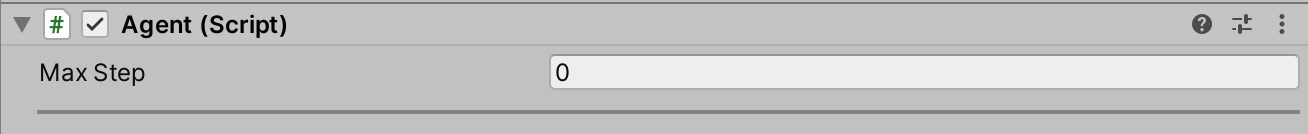
\includegraphics[scale=0.5]{img/agent_komponente}
  \caption{Unity ML-Agents Agenten Komponente}
  \label{fig:agent_komponente}
\end{figure}

Abbildung \ref{fig:agent_komponente} zeigt die Basiskomponente des Agenten. Die Agenten Komponente stellt alle grundlegenden Funktionen des verstärkenden Lernens bereit und implementiert die Verbindung zur Akademie und dem Verhalten des Agenten. Ohne das überschreiben der Funktionen ist die Agentenklasse jedoch ohne Funktion. Die genauen Methoden zur Implementierung eigener Agentenklassen werden näher in Kapitel \ref{subsec:programmierschnittstellen} behandelt. Das einzige Feld zur Konfiguration ist Max Step, welches die maximale Anzahl der Schritte innerhalb einer Episode festlegt.

\begin{figure}[H]
  \centering  
  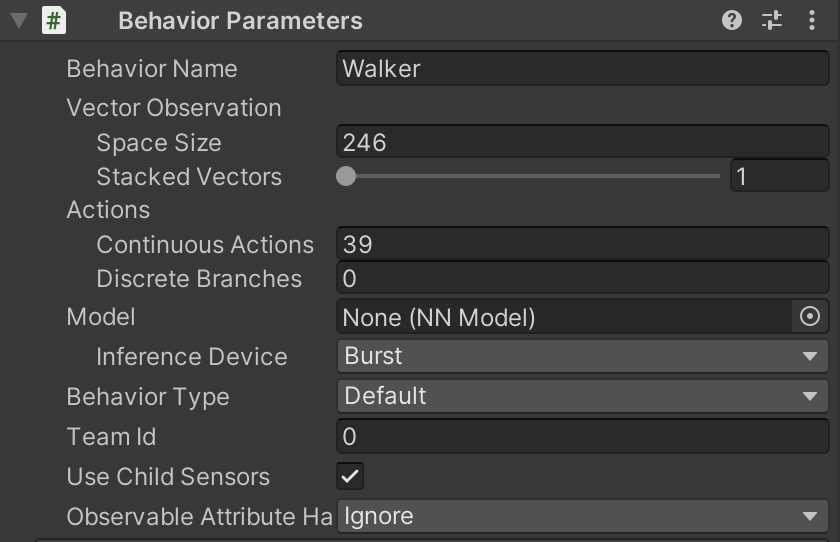
\includegraphics[scale=0.5]{img/verhalten_komponente.png}
  \caption{Unity ML-Agents Verhalten Parameter Komponente}
  \label{fig:verhalten_komponente}
\end{figure}

In Abbildung \ref{fig:entscheidung_anfragen_komponente} ist die Verhaltens Parameter Komponente zusehen. Das Verhalten legt die Ein- und Ausgangsgröße des Modells fest. Für das Training muss ein gleichnamiges Verhalten in der Konfigurationsdatei definiert sein. Um ein bereits trainiertes Verhalten zu verwenden muss im Modell Feld die Modelldatei referenziert werden.

\begin{itemize}
  \item Behaviour Name: Name des Verhaltens / wird in Trainer Konfiguration referenziert
  \item Space Size: Anzahl an Beobachtungen / Inputknoten für NN
  \item Continuous Actions: Anzahl an Aktionen / Outputknoten von NN
  \item Model: Referenz auf bereits trainiertes Modell zur Verwendung in Inferenz
  \item Behaviour Type: Lernmodus Default = Lernen, Heuristic, Inferenz
\end{itemize}

\begin{figure}[H]
  \centering  
  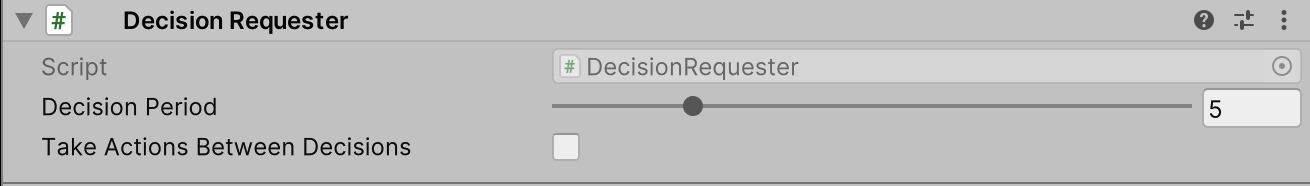
\includegraphics[scale=0.5]{img/entscheidung_anfragen_komponente.png}
  \caption{Unity ML-Agents Entscheidung Anfragen Komponente}
  \label{fig:entscheidung_anfragen_komponente}
\end{figure}

Die Komponente in Abbildung \ref{fig:entscheidung_anfragen_komponente} fragt in regelmäßigen Abständen Entscheidungen an. Das bedeutet es wird eine Beobachtung erstellt. Darauf wird die Beobachtung als Eingangswert für das neuronale Netz genutzt und dann eine Aktion vom neuronalen Netz ausgewählt. Während dem training wird diese Beobachtung zusammen mit der darauf ausgeführten Aktion und der resultierenden Belohnung im Trainingsspeicher abgelegt. Die "Decision Period" gibt an in welchem Interval der Agent eine Entscheidung treffen soll. Das "Kontrollkästchen Take Actions Between Decisions" gibt an ob der Agent die ausgewählte Aktion wiederholen soll bis die nächste Aktion ausgewählt wurde.

\subsection{Programmierschnittstellen}
\label{subsec:programmierschnittstellen}
Die Agenten Komponente enthält einige Funktionen die für das Training eines Agenten implementiert werden müssen. In den folgenden Absätzen werden die Funktionen anhand Beispielen näher erklärt.

\begin{lstlisting}[caption={Agent Funktionen},captionpos=b,label={lst:agent_funktionen}]
public override void CollectObservations(VectorSensor sensor)
{
    sensor.AddObservation(floatObservation);
}

public override void OnActionReceived(ActionBuffers actionBuffers)
{
    var continuousActions = actionBuffers.ContinuousActions;
    movement.x += continuousActions[0]
    movement.y += continuousActions[1]
}

public virtual void FixedUpdate()
{
    AddReward(floatReward);
}
\end{lstlisting}

In der CollectObservations Methoden wird festgelegt welche Daten dem Agent für das Training bereit stehen siehe Listing \ref{lst:agent_funktionen} Zeile 1-3. CollectObservations wird für jede angefragte Entscheidung ausgeführt und das Ergebnis an das NN Modell oder den Python Trainer übergeben.

Wenn eine Entscheidung angefragt wurde und das NN Modell ein Ergebnis liefert wird dieses hier von numerischen Werten in Aktionen umgewandelt. In Listing \ref{lst:agent_funktionen} Zeile 6-11 wird gezeigt wie die Aktion in x und y Bewegung umgesetzt wird.

Im Beispielcode in Listing \ref{lst:agent_funktionen} Zeile 13-16 wird ein Reward in jedem FixedUpdate vergeben über die AddReward Methode die auch Teil der Agenten-Komponente ist. Der Reward kann aber an jeder Stelle im Code vergeben werden, der Code dient hier nur als ein Beispiel.

\begin{lstlisting}[caption={Trainer Konfigurationsdatei},captionpos=b,label={lst:trainer_konfiguration}]
{
behaviors:
  Walker:
    trainer_type: ppo
    hyperparameters:
      batch_size: 2048
      buffer_size: 20480
      learning_rate: 0.0003
      beta: 0.005
      epsilon: 0.2
      lambd: 0.95
      num_epoch: 3
      learning_rate_schedule: linear
    network_settings:
      normalize: true
      hidden_units: 256
      num_layers: 3
      vis_encode_type: simple
    reward_signals:
      extrinsic:
        gamma: 0.995
        strength: 1.0
    keep_checkpoints: 5
    checkpoint_interval: 5000000
    max_steps: 30000000
    time_horizon: 1000
    summary_freq: 30000
environment_parameters:
  environment_count: 100.0
}
\end{lstlisting}

Die Trainings Konfigurationsdatei (siehe Listing \ref{lst:trainer_konfiguration}) enthält mehrere Teile. Der Hyperparameter Teil enthält die Hyperparameter des Maschinellen Lernalgorithmuses (Zeile 5-13), danach folgt der network\_settings Teil welcher die Konfiguration des Neuronalennetzes festlegt (Zeile 14-18). Anschließend folgen noch Konfigurationen für die Belohnungssignale im Bereich reward\_signals (Zeile 19-22) und Einstellungen für die Speicherung der Daten sowie der länge des Trainings (Zeile 23-27). Ganz am Ende der Konfigurationsdatei (Zeile 28-29) befinden sich noch Umgebungsparameter welche erweitert und während dem Training ausgelesen werden können.


\section{Unity Physik}
\label{sec:physik}
Unitys eingebaute Physik-Engine ermöglicht die realistische Berechnung von Kollisionen, Schwerkraft und anderen Kräften, was Entwicklern hilft, immersive und interaktive Umgebungen zu schaffen.

Die Festkörperkomponente (Rigidbody) erlaubt es, 3D-Objekte als nicht verformbare Einheiten innerhalb dieses Systems zu simulieren. Dies ist entscheidend für die Entwicklung realistischer physikalischer Interaktionen, wie z. B. das Bewegen von Objekten, die auf Kräfte, Drehmomente und Kollisionen reagieren.

\begin{figure}[H]
  \centering  
  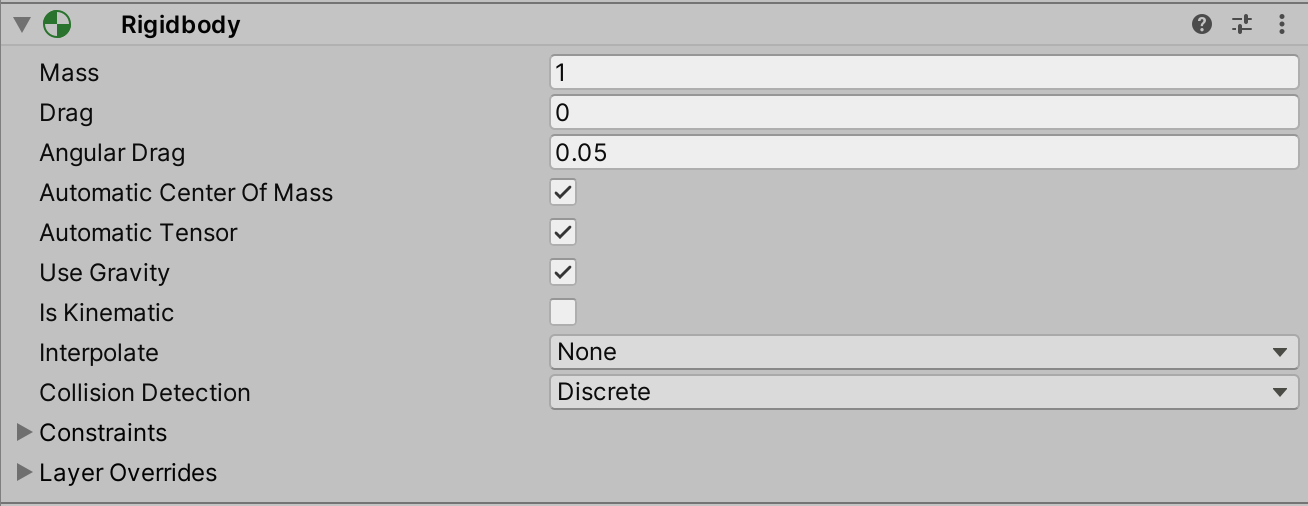
\includegraphics[scale=0.5]{img/komponente_rigidbody.png}
  \caption{Unity ML-Agents Physik Festkörper}
  \label{fig:komponente_rigidbody}
\end{figure}
\begin{itemize}
  \item Mass: gibt das Gewicht des Körpers an
  \item Drag: definiert den Geschwindigkeitsverlust eines Körpers in Bewegung durch Reibung, Luftwiederstand
  \item Angular Drag: definiert den Geschwindigkeitsverlust eines Körpers für Rotationsbewegung
  \item Collision Detection: legt fest wie Kollisionen berechnet werden (Akkurat/Leistung)
 \end{itemize}
 
Um Kollisionen zwischen Objekten zu berechnen benötigen diese zusätzlich eine Kollisionskomponente. Komplexe 3D-Modelle können in der Kollisionsberechnung jedoch in ihrer direkten Form rechenintensiv sein. Zur Optimierung werden diese Modelle vereinfacht, indem sie durch geometrische Formen wie Kugeln, Kapseln oder Boxen dargestellt werden. Abbildung \ref{fig:komponente_collider} zeigt die Unterschiedlichen Kollisionskomponenten in Unity. Abbildung \ref{fig:charakter_mixamo_collider} zeigt wie die Kollisionkomponenten (gelbe Wireframes) genutzt werden um die Körperteile eines komplexen 3D Modells vereinfacht abzubilden.

 \begin{figure}[H]
  \centering  
  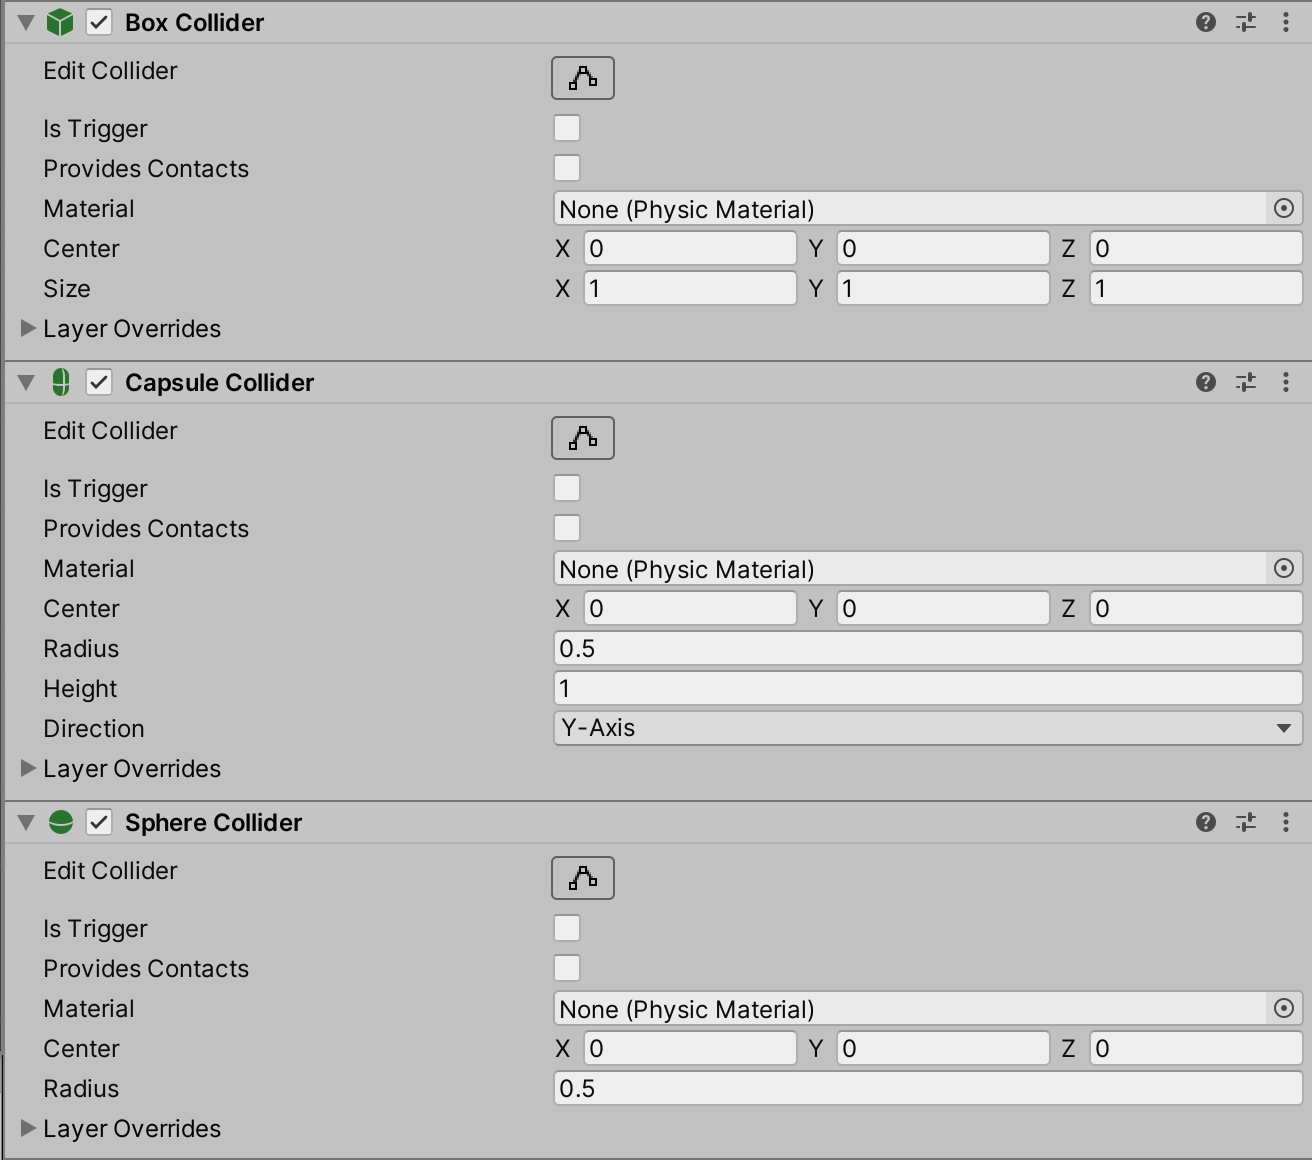
\includegraphics[scale=0.5]{img/komponente_collider.png}
  \caption{Unity ML-Agents Physik Kollisionskomponenten}
  \label{fig:komponente_collider}
\end{figure}

 \begin{figure}[H]
  \centering  
  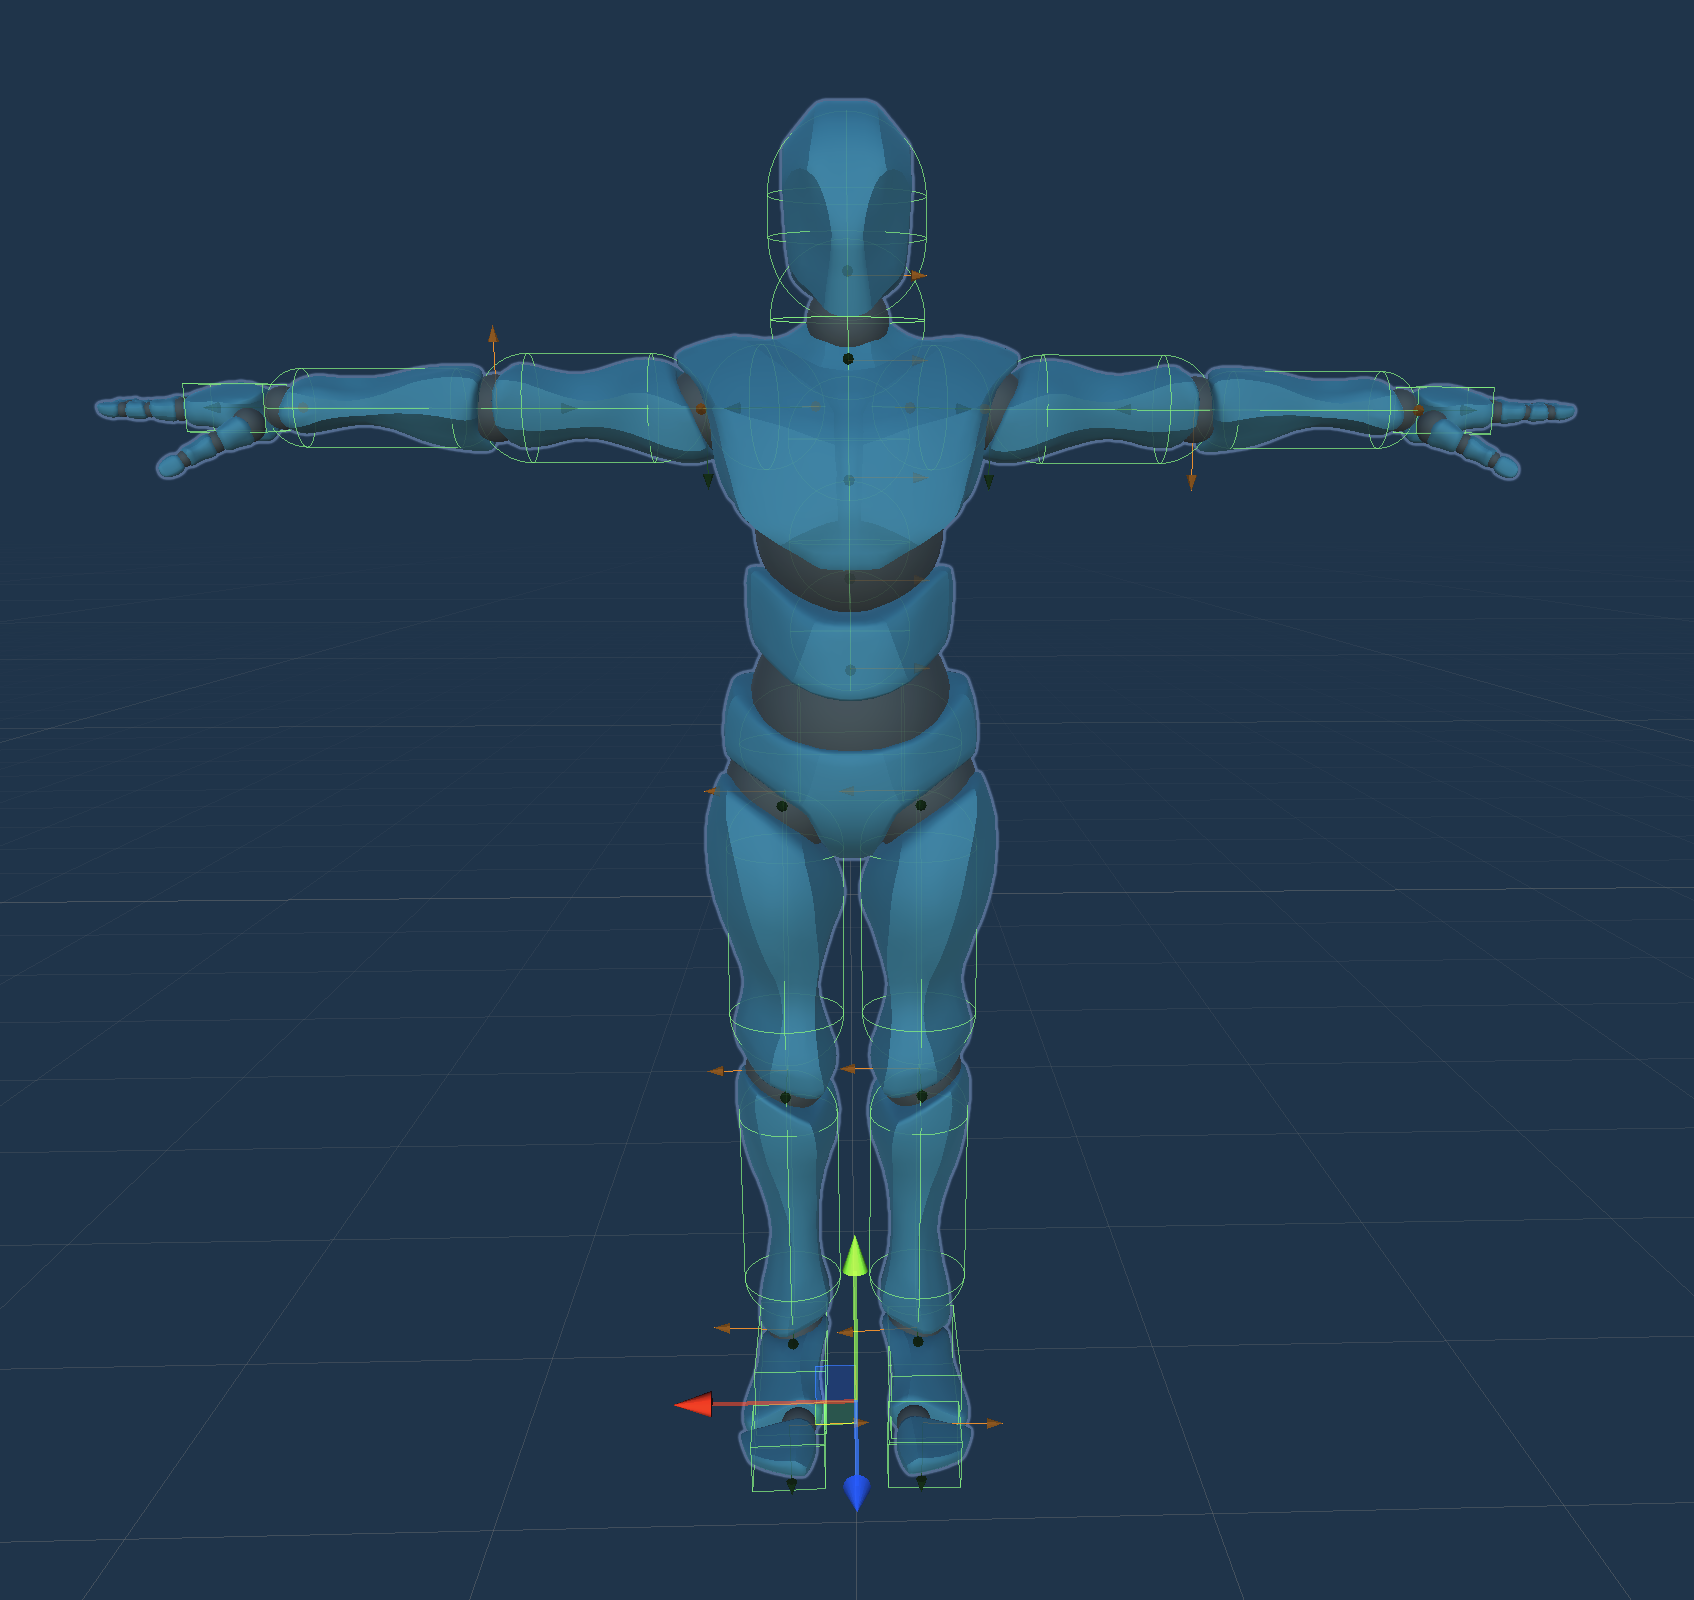
\includegraphics[scale=0.4]{img/charakter_mixamo_collider.png}
  \caption{Unity ML-Agents Physik Charakter vereinfacht mit Kollisionskomponenten }
  \label{fig:charakter_mixamo_collider}
\end{figure}

Festkörper können mit Gelenken zu komplexeren Körperstrukturen verbunden werden. Die Konfigurierbare Gelenkkomponente (Configurable Joint) ermöglicht die Simulation von Gelenken mit freier Bewegung und Rotation auf allen drei Achsen. Dies ist wesentlich, um realistische Animationen und Interaktionen in Softwaresimulationen zu erzeugen. Im Kontext dieser Arbeit wird das Gelenk auf Rotation beschränkt und als kugelförmiges Gelenk verwendet. Die Gelenke einer humanoiden Figur können somit vereinfacht aber ausreichend genau simuliert werden.

\begin{figure}[H]
  \centering
  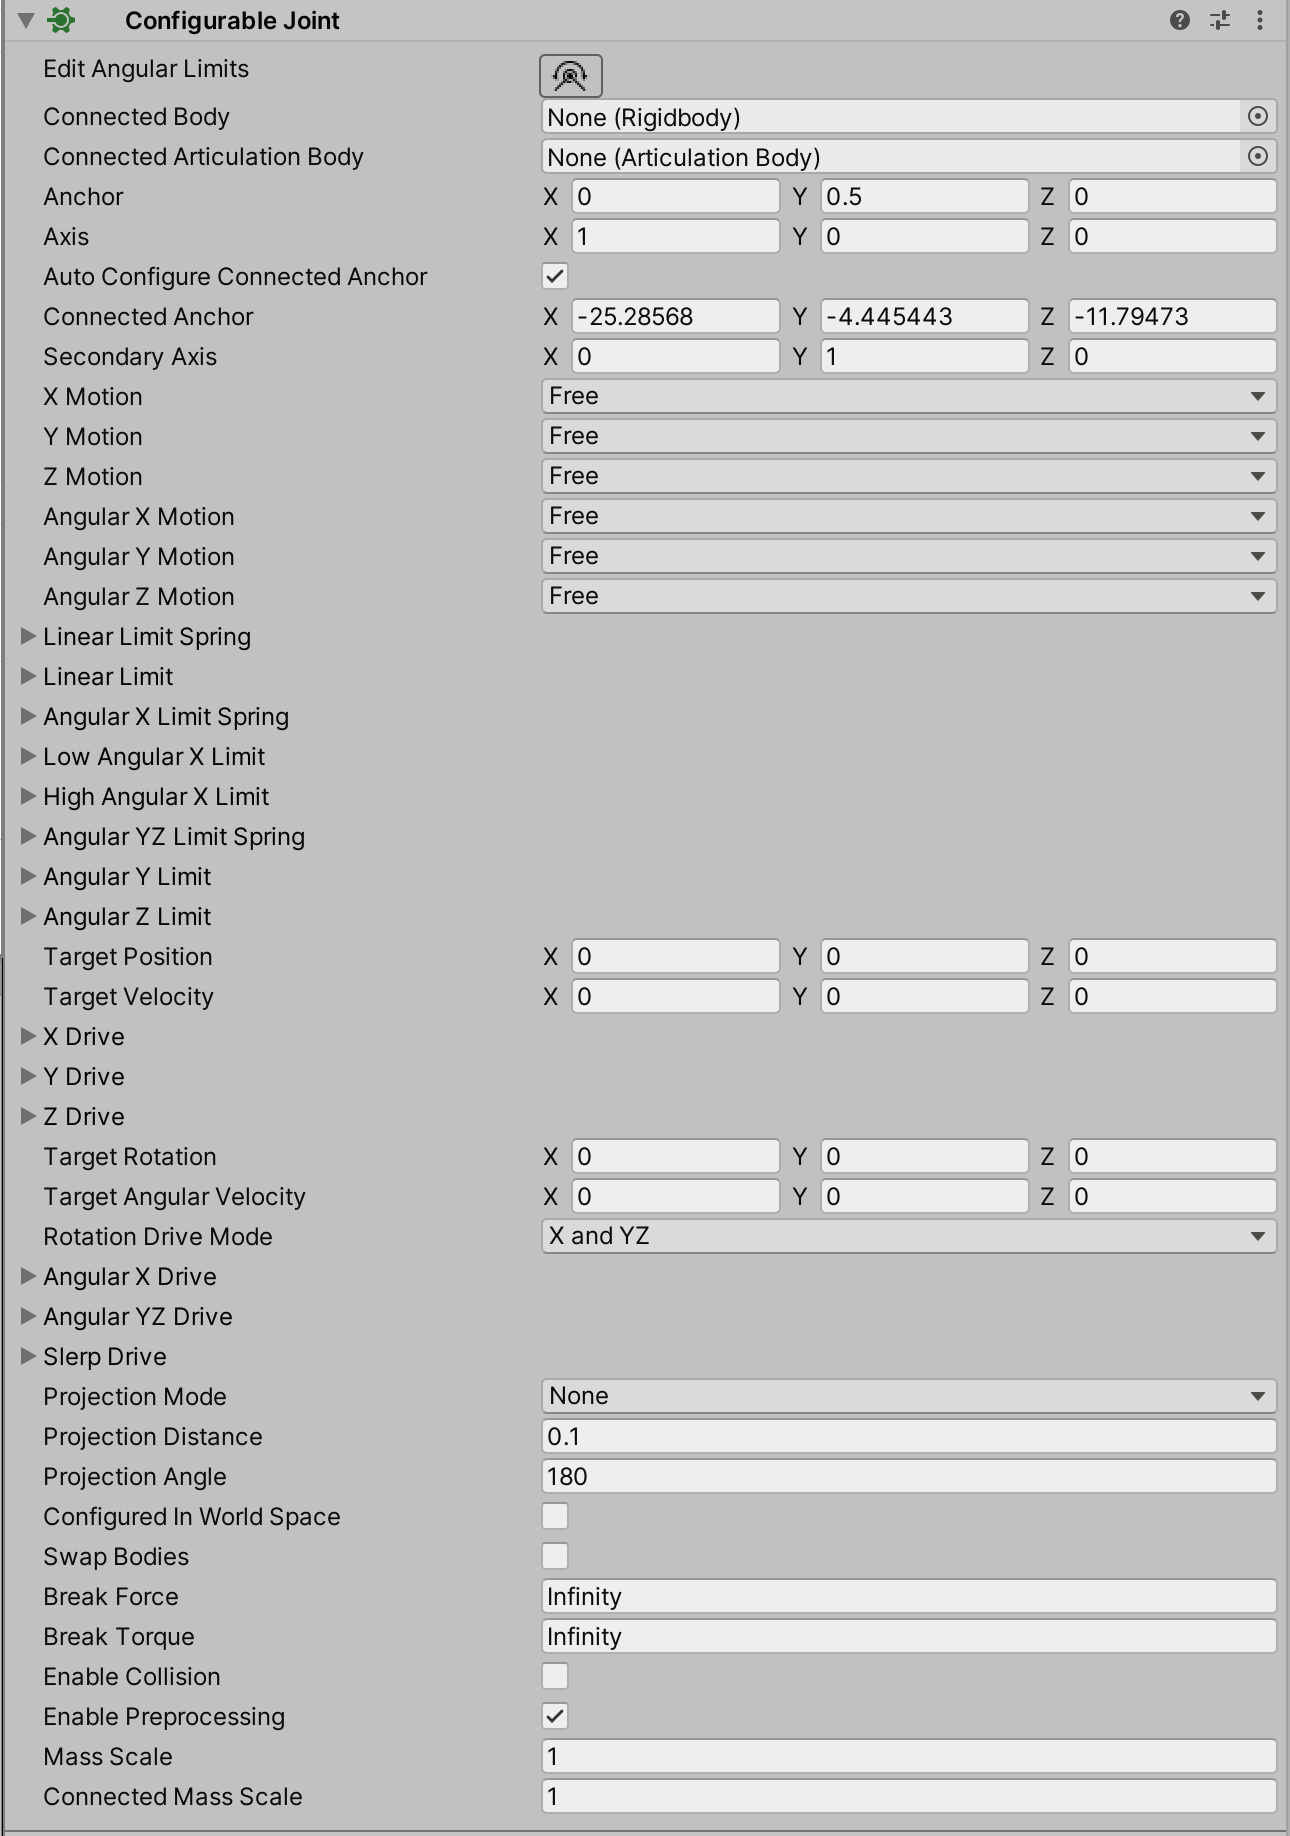
\includegraphics[scale=0.5]{img/komponente_configurable_joint.png}
  \caption{Unity ML-Agents Physik Gelenk}
  \label{fig:komponente_configurable_joint}
\end{figure}
\begin{itemize}
  \item Connected Body: bestimmt, mit welchem Körper das Gelenke verbunden ist
  \item Anchor: legt fest, an welchem Punkt die Verbindung zum verbundenen Körper besteht
  \item Axis: legt die Hauptbewegungs- und Rotationsachse fest
  \item Secondary Axis: legt die sekundäre Beweungs- und Rotationsachse fest
  \item Angular X Y Z Motion: bestimmt, ob das Gelenk Rotation zwischen den Körpern auf der X Y Z Achse zulässt
  \item Target Position: bestimmt das Ziel, zu welchem das Gelenk sich bewegen soll
  \item Angular X Y Z Limit: ermöglicht das Festlegen von Winkellimits für die Rotationsbewegungen
  \item X Y Z  und Slerp Drive: bestimmen die Stärke der Federkraft welche das Gelenk in die Zielposition bewegt
\end{itemize}
{\chapter{Analyse}}
\label{sec:analyse}
Zusätzlich zu den maschinellen Lernkomponenten liefert Unity auch Demonstrationsumgebungen, in denen verschiedene Lösungen für gängige Verstärkungslernprobleme implementiert sind. In der Walker-Demo wird ein physisch simulierter Charakter darauf trainiert, zu einem Zielwürfel zu laufen. Diese Demo-Umgebung implementiert bereits einige Grundlagen für die Steuerung eines physisch simulierten Charakters. Aus diesem Grund wird in dieser Arbeit die Walker-Demo als Grundlage für die Entwicklung genutzt. In diesem Kapitel wird daher die Walker-Demo analysiert, um in den folgenden Kapiteln darauf aufzubauen.

\section{Szenenaufbau}

\begin{figure}[H]
  \centering  
  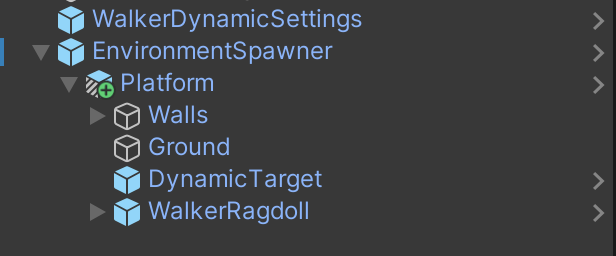
\includegraphics[scale=0.8]{img/walker_demo_hierarchy.png}
  \caption{Walker-Demo Hierarchy}
  \label{fig:walker_demo_hierarchy}
\end{figure}

\begin{figure}[H]
  \centering  
  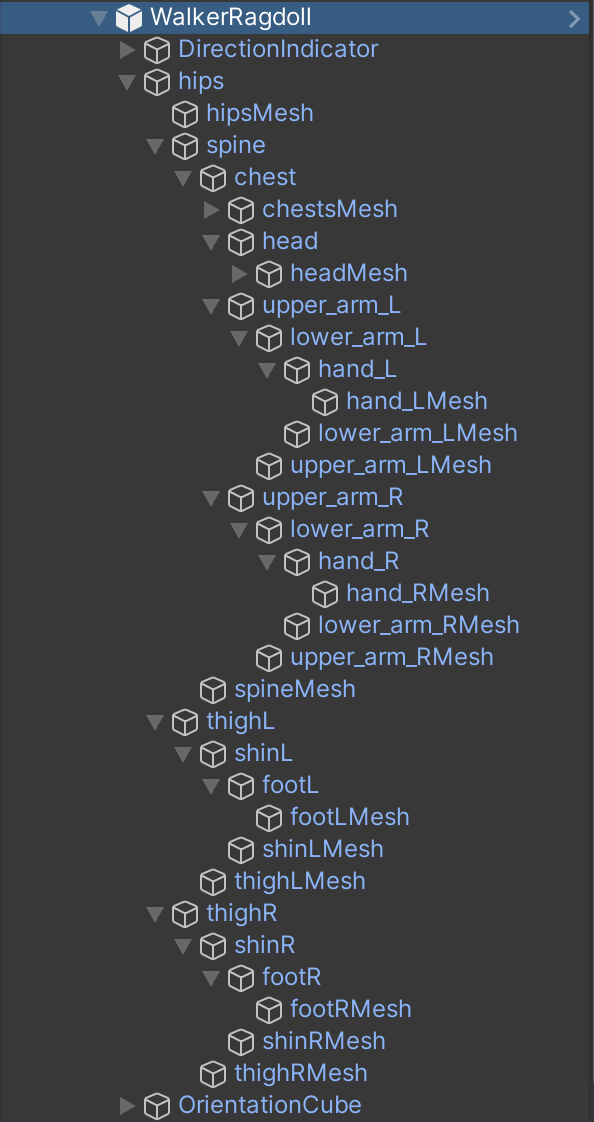
\includegraphics[scale=0.5]{img/agent_hierarchy.png}
  \caption{Agent Hierarchy}
  \label{fig:agent_hierarchy}
\end{figure}


\section{Physikkomponenten und -konfiguration}
Der Körper besteht aus 11 Kapseln, drei Kugeln und 2 Quadern, jeder dieser Formen hat eine Festkörper und eine Kollisions Physikkomponente. Zwischen den Körperteilen werden die Gelenke als Kugelgelenke simuliert.

\begin{center}
{\rowcolors{2}{lightgray}{gray!50!lightgray!50}
\begin{tabular}{ |p{3cm}|p{3cm}|p{2cm}|p{4cm}|p{2cm}| }
\hline
Körperteil& Verbundenes Körperteil & Gewicht & Winkellimits & Form \\
\hline
Hüfte & - & 15kg & - & Kapsel \\
Wirbelsäule & Hüfte & 10kg & x(-20,20) y(-20,20) z(-15,15) & Kapsel \\
Oberkörper & Wirbelsäule & 8kg & x(-20,20) y(-20,20) z(-15,15) & Kapsel \\
Kopf & Oberkörper & 6kg & x(-30,10) y(-20,20) & Kugel \\
Oberarm LR & Oberkörper & je 4kg & x(-60,120) y(-100,100) & Kapsel \\
Unterarm LR & Oberarm & je 3kg & x(0,160) & Kapsel \\
Hand LR & Unterarm & je 2kg & - & Kugel \\
Oberschenkel LR & Hüfte & je 14kg& x(-90,60) y(-40,40) & Kapsel \\
Unterschenkel LR & Oberschenkel & je 7kg &  x(0,120) & Kapsel \\
Fuß LR & Unterschenkel & je 5kg & x(-20,20 y(-20,20) z(-20,20) & Quader \\
\hline
\end{tabular}}
\end{center}

\section{Agent implementierung}
lernablauf (Beobachtung, Aktionen ausführen, Belohnungsfunktion, einrichtung)

\begin{figure}[H]
  \centering  
  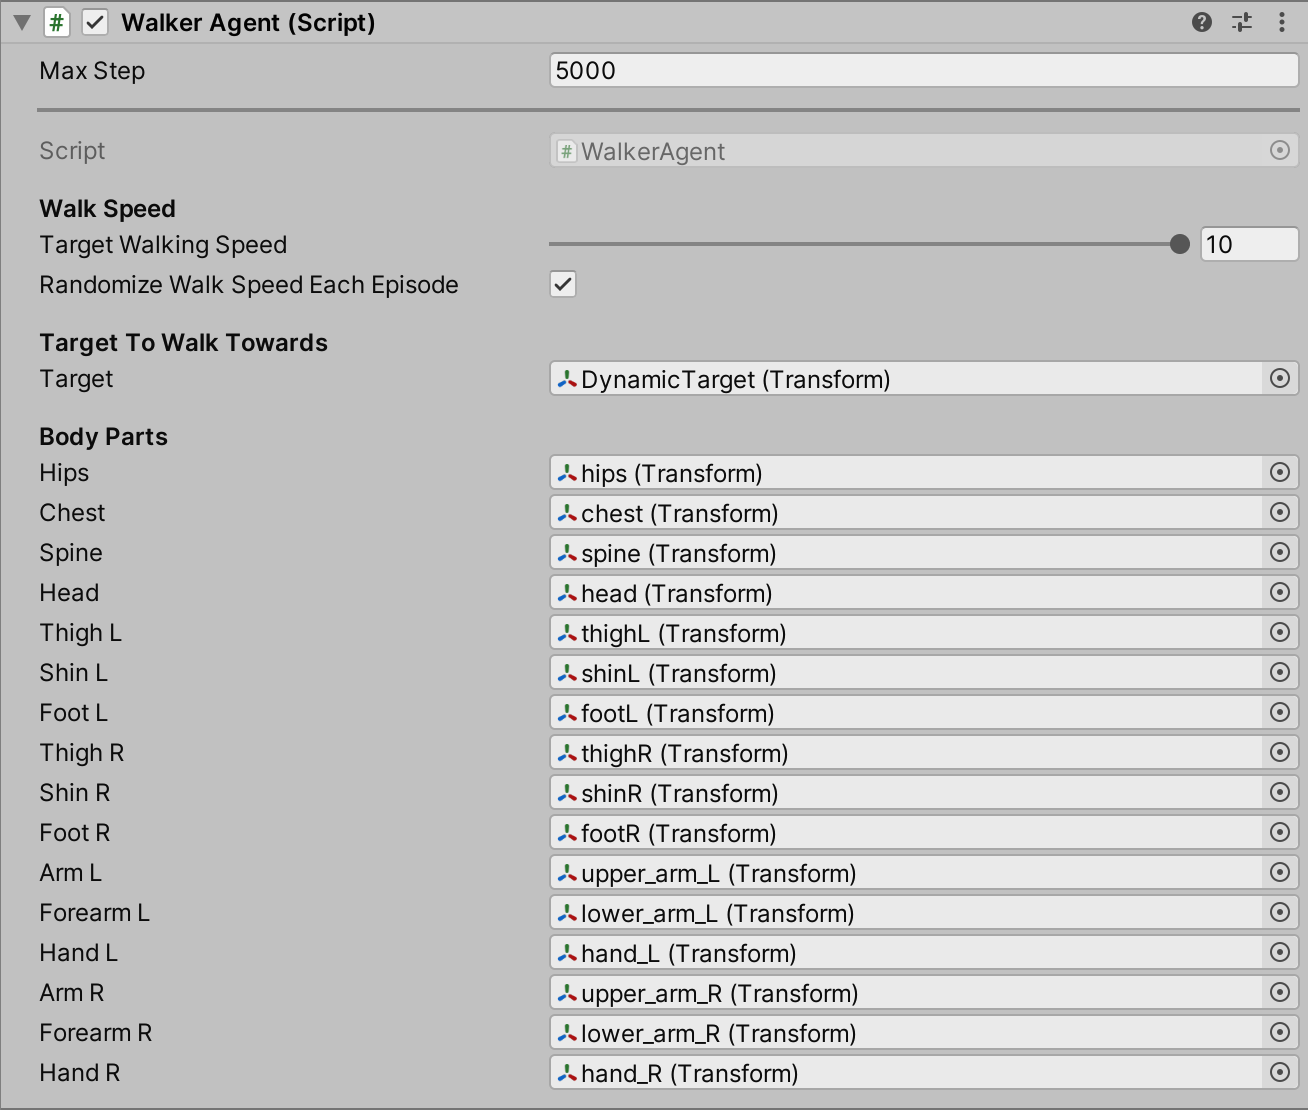
\includegraphics[scale=0.5]{img/agent_konfiguration.png}
  \caption{Agent Konfiguration}
  \label{fig:agent_konfiguration}
\end{figure}

Agent Code hier einfügen? oder evtl. im Anhang?

\section{Ziel}
Ziele (target controller)

{\chapter{Fazit}}
\label{sec:fazit}
Text

\appendix
\chapter{Anhang 1}

%Literaturverzeichnis
\printbibliography[title=Literaturverzeichnis]

\end{document}
